% Uncomment this to make slides with overlays:
%\documentclass[slides]{beamer}

% Uncomment these (but comment the above \documentclass line) to make handouts:
\documentclass[handout]{beamer}

% Uncomment these to have more than one slide per page
\usepackage{pgfpages}
\pgfpagesuselayout{2 on 1}[border shrink=5mm]
\pgfpageslogicalpageoptions{1}{border code=\pgfusepath{stroke}}
\pgfpageslogicalpageoptions{2}{border code=\pgfusepath{stroke}}

\usepackage[]{graphicx, color, hyperref}

\mode<presentation>
{
	%\usetheme[secheader]{Boadilla}
	%\usecolortheme[rgb={.835, .102,.169}]{structure}  
	\usetheme[width= 0cm]{Goettingen}
	%\setbeamercovered{transparent}
}
\setbeamertemplate{navigation symbols}{}
\setbeamertemplate{footline}[frame number]

\definecolor{blue2}{rgb}{0.278,0.278,0.729} 
\newcommand{\blue}[1]{\textcolor{blue2}{#1}}
\newcommand{\white}[1]{\textcolor{white}{#1}}
\newcommand{\red}[1]{\textcolor{red}{#1}}
\newcommand{\xbar}{\overline{x}}
\newcommand{\ybar}{\overline{y}}
\newcommand{\phat}{\widehat{p}}
\newcommand{\prob}{\mbox{Pr}}
\newcommand{\E}{\mathbb{E}}
\newcommand{\Var}{\mbox{Var}}
\newcommand{\cp}{\oplus}
\newcommand{\cm}{\circleddash}


\title{Lecture 2: Sampling and Bias}
\author{Chapter 1.3}
\date{}


\begin{document}
%------------------------------------------------------------------------------
\begin{frame}
\titlepage
\end{frame}
%------------------------------------------------------------------------------


%------------------------------------------------------------------------------
\begin{frame}
\frametitle{Goals for Today}
\begin{itemize}
  \item Understand important considerations about data collection in particular \blue{sampling}.
  \item Two real-world examples.
  \item Food for thought about the next lecture: explanatory/response variables and causality.  
\end{itemize}

\end{frame}
%------------------------------------------------------------------------------


%------------------------------------------------------------------------------
\begin{frame}
\frametitle{Recall:  What is statistics?}

The general scientific process of investigation can be summed up as follows:

\begin{enumerate}
\item Identify the scientific question or problem
\item Collect relevant data on the topic
\item Analyze the data
\item Form a conclusion and communicate it
\end{enumerate}

\pause Point 2 is just as, if not, more important than point 3.

\end{frame}
%------------------------------------------------------------------------------


%------------------------------------------------------------------------------
\begin{frame}
\frametitle{Populations and Samples}
We want to make statements about some aspect of a \blue{study/target population}.  

\begin{enumerate}
\item What proportion of Vermonters smoke?
\item What are the sexual behaviors of males and female Americans in 1948?
\end{enumerate}

\end{frame}
%------------------------------------------------------------------------------


%------------------------------------------------------------------------------
\begin{frame}
\frametitle{Populations and Samples}

It is often not feasible to collect data for every case in the population.  If so, we take a \blue{sample} of cases.

\begin{center}
\pause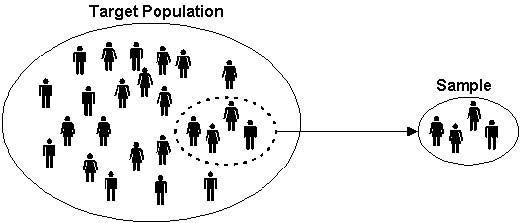
\includegraphics[width=3in]{./figure/target-population.jpg} 
\end{center}

\pause 

Important:
%
% Comment this
%
%\begin{itemize}
%\item If the sample is \blue{representative} of the target population, then the sample's results will be \blue{generalizable}.  
%\item If you want your sample to be \blue{representative}, you need to \blue{randomly} sample from the entire target population.  
%\end{itemize}

\end{frame}
%------------------------------------------------------------------------------


%------------------------------------------------------------------------------
\begin{frame}
\frametitle{Populations and Samples}
So say we take we collect a sample of 100 Vermonters and poll their smoking habits in two ways:

\begin{itemize}
\pause\item We stand outside a tobacco store and randomly select 100 people walking nearby.  This is a non-representative sample AKA a \blue{biased sample}.
\pause\item We have a list of all citizens of the state and randomly select 100 people from this list.  This sample is representative and hence the poll's results can generalize to all of VT.  
\end{itemize}

\end{frame}
%------------------------------------------------------------------------------


%------------------------------------------------------------------------------
\begin{frame}
\frametitle{Comment on the Representativeness of These Samples:}

\begin{small}
\begin{enumerate}
\item The Royal Air Force wants to study how resistant their airplanes are to bullets. They study the bullet holes on all the airplanes on the tarmac after an air battle against the Luftwaffe (German Air Force).
\item I want to know the average income of Reed graduates in the last 10 years.  So I get the records of 10 randomly chosen Reedies.  They all answer and I take the average.
\item Imagine it's 1993 i.e. almost all households have landlines.  You want to know the average number of people in each household in Portland.  You randomly pick out 500 phone numbers from the phone book and conduct a phone survey.
\item You want to know the prevalence of illegal downloading of TV shows among Reed students.  You get the emails of 100 randomly chosen Reedies and ask them ``How many times did you download a pirated TV show last week?''
\end{enumerate}
\end{small}

\end{frame}
%------------------------------------------------------------------------------




%------------------------------------------------------------------------------
\begin{frame}
\frametitle{Statistics in Society: Alfred Kinsey}
In the mid 20th century, biologist/sexologist Alfred Kinsey wanted to study human sexuality.  

\begin{center}
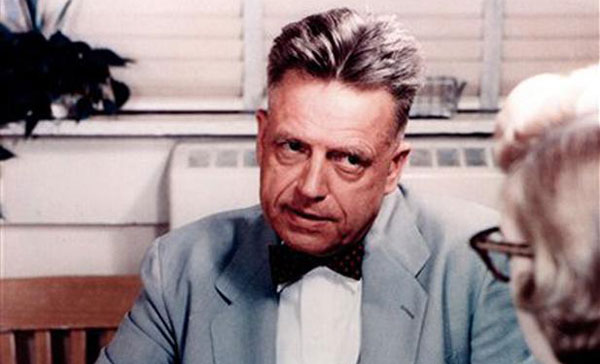
\includegraphics[width=0.4\textwidth]{./figure/alfred-kinsey.jpg}
\end{center}

\pause At the time sexuality was an extremely taboo subject, very little research had been conducted at that point and Kinsey was astonished at the public's general ignorance.  

\end{frame}
%------------------------------------------------------------------------------



%------------------------------------------------------------------------------
\begin{frame}
\frametitle{Statistics in Society: Kinsey's Questions/Research Problem}
What type of questions was Kinsey interested in?  Using his 300 question survey, he hoped to address...

\begin{enumerate}
\pause \item What percentage of Americans engaged in premarital and extramarital sex?
\pause \item What were the homosexual tendencies of American males?
\pause \item How common were oral sex and masturbation?
\item $\ldots$
\end{enumerate}
\end{frame}
%------------------------------------------------------------------------------



%------------------------------------------------------------------------------
\begin{frame}
\frametitle{Statistics in Society: Kinsey Reports}
The results were published two books on human sexual behavior known as the ``Kinsey Reports'': Sexual Behavior in the Human Male (1948) and Female (1953).  

\begin{center}
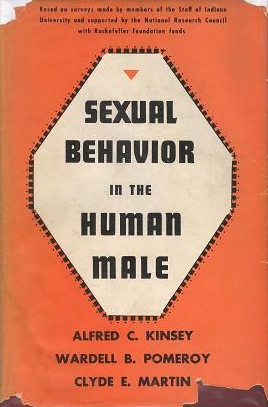
\includegraphics[width=0.4\textwidth]{./figure/kinsey_male.jpg}
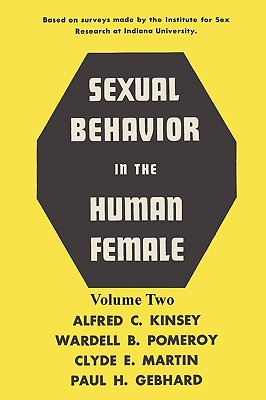
\includegraphics[width=0.4\textwidth]{./figure/kinsey_female.jpg}
\end{center}

\end{frame}
%------------------------------------------------------------------------------



%------------------------------------------------------------------------------
\begin{frame}
\frametitle{Statistics in Society: Conclusions of Kinsey Reports}

Kinsey claimed, among other things
\begin{enumerate}
	\pause \item 85\% of white men had had premarital sex, 50\% had had extra-marital sex
	\pause \item Kinsey wrote in 1948 that \blue{one in ten} white men were more or less, exclusively homosexual for at least three years between the ages of 16 and 55.
	\pause \item Kinsey reported that oral sex was very common (70\% of couples did it), masturbation was very common (almost 63\%/92\% of women/men did it)
\end{enumerate}

\end{frame}
%------------------------------------------------------------------------------



%------------------------------------------------------------------------------
\begin{frame}
\frametitle{Statistics in Society: Reaction to Kinsey Reports}
Needless to say, people were taken quite aback.  
\begin{center}
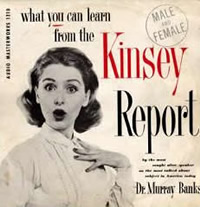
\includegraphics[height=4cm]{./figure/kinsey_report1.jpg}
\hspace{0.5cm}
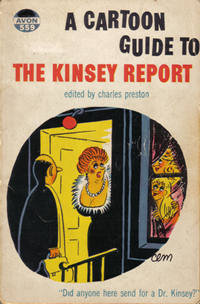
\includegraphics[height=4cm]{./figure/kinsey_report2.png}
\end{center}
There was also a huge conservative backlash against the reports.  

\end{frame}
%------------------------------------------------------------------------------



%------------------------------------------------------------------------------
\begin{frame}
\frametitle{Statistics in Society: Kinsey's Methods}
What were his data collection methods?  How did he sample his data? Focusing on the male report, my understanding is that 

\begin{enumerate}
\pause \item He did in fact base his conclusions on a very large sample size of 5300 males.
\pause \item He sought out volunteers to answer his 300 question survey.
\pause \item He recruited new people by asking previous respondents if they knew other people.  This led to a large proportion of his sample to include prison populations and male prostitutes.  
\end{enumerate}

\pause \blue{What could be some issues?}

\end{frame}
%------------------------------------------------------------------------------


%------------------------------------------------------------------------------
\begin{frame}
\frametitle{Response of the American Statistical Association}
The American Statistical Association criticized the sampling procedure.  In particular, John Tukey, one of the most eminent statisticians of the time, said

\vspace{0.5cm}

\begin{quotation}
\pause \blue{``A random selection of three people would have been better than a group of 300 chosen by Mr. Kinsey.''}
\end{quotation}

\vspace{0.5cm}

\pause Even though the Kinsey Report was groundbreaking and contributed much to the field of sexology by bringing many topics to the forefront, Kinsey's statements were not generalizable to the general public.  

\end{frame}
%------------------------------------------------------------------------------


%%------------------------------------------------------------------------------
%\begin{frame}
%\frametitle{Reed Campus Climate Survey}
%
%During the 2012-2013 academic year Reed contracted Rankin \& Associates Consulting to conduct the Campus Climate Survey to ``examine the learning, living, and working environment at Reed College.''
%
%\vspace{0.5cm}
%
%\pause On page v and iii of the Executive Summary: \blue{\href{http://www.reed.edu/institutional\_diversity/campus\_climate.html}{http://www.reed.edu/institutional\_diversity/campus\_climate.html}}
%
%
%\end{frame}
%%------------------------------------------------------------------------------


%------------------------------------------------------------------------------
\begin{frame}
\frametitle{Examples of Different Types of Bias:}

%
% Comment this
%
%\begin{enumerate}
%\item \blue{Volunteer bias}:  individuals who are more willing to participate have a higher chance of being sampled.
%\item \blue{Survival bias}:  large segments of the population who ``died'' are not sampled.
%\item \blue{Convenience sample bias}:  individuals who are easily accessible are more likely to be included.
%\end{enumerate}
%
%All the above are instances of \blue{selection bias}: some individuals are more likely to be selected for study than others.

\end{frame}
%------------------------------------------------------------------------------



%------------------------------------------------------------------------------
\begin{frame}
\frametitle{Moral of the Story}
For you:
\begin{enumerate}
\pause \item \blue{the consumer of statistics}: Ask yourself what was the study design?
\begin{itemize}
\item Who is the study population?
\item Who are the respondents and how were they selected?
\end{itemize}
\pause \item \blue{the producer of statistics}:  If you want your results to generalize \blue{beyond} just your sample to your study population, your sampling scheme has to as representative as feasible.
\end{enumerate}

\end{frame}
%------------------------------------------------------------------------------


%------------------------------------------------------------------------------
\begin{frame}
\frametitle{Another Example: Facebook}

In the news
\begin{itemize}
\item NPR's story on younger users \blue{\href{http://www.npr.org/2014/01/09/261108836/many-younger-facebook-users-unfriend-the-network}{(link)}}
\item Facebook Envy \blue{\href{http://psychcentral.com/blog/archives/2015/04/09/the-psychology-of-facebook-depression-avoid-social-comparisons-envy/}{(link)}}
\end{itemize}

\pause \vspace{1cm}

Let's consider a hypothetical scenario where we compare 15 life occurrences between you and your friend rated between 0 (lowest) and 5 (highest).

\end{frame}
%------------------------------------------------------------------------------


%------------------------------------------------------------------------------
\begin{frame}
\frametitle{Another Example: Facebook}

\begin{center}
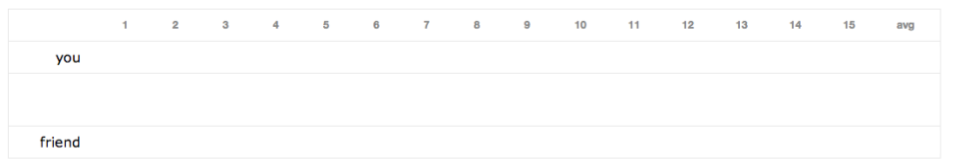
\includegraphics[width=\textwidth]{./figure/FB1}
\end{center}

\textcolor{white}{The selective ``Facebook image curation'' your friend performed is a form of selection bias!}

\end{frame}
%------------------------------------------------------------------------------


%------------------------------------------------------------------------------
\begin{frame}
\frametitle{Another Example: Facebook}

\begin{center}
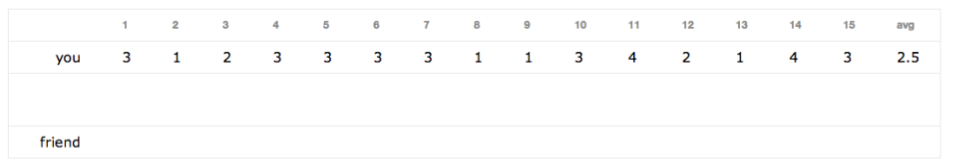
\includegraphics[width=\textwidth]{./figure/FB2}
\end{center}

\textcolor{white}{The selective ``Facebook image curation'' your friend performed is a form of selection bias!}

\end{frame}
%------------------------------------------------------------------------------


%------------------------------------------------------------------------------
\begin{frame}
\frametitle{Another Example: Facebook}

\begin{center}
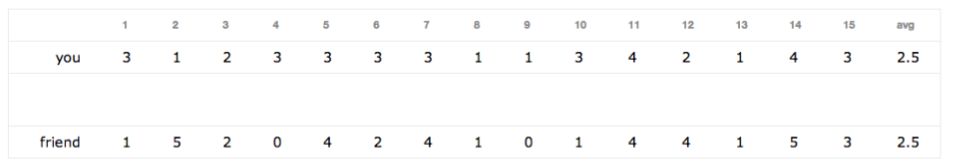
\includegraphics[width=\textwidth]{./figure/FB3}
\end{center}

\textcolor{white}{The selective ``Facebook image curation'' your friend performed is a form of selection bias!}

\end{frame}
%------------------------------------------------------------------------------


%------------------------------------------------------------------------------
\begin{frame}
\frametitle{Another Example: Facebook}

\begin{center}
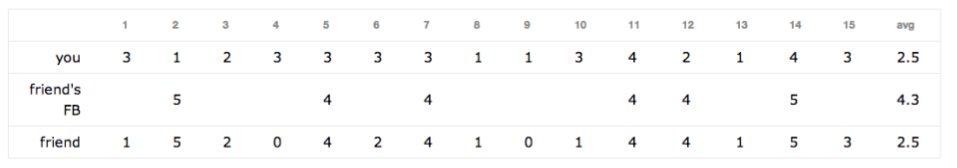
\includegraphics[width=\textwidth]{./figure/FB4}
\end{center}

\pause The selective ``Facebook image curation'' your friend performed is a form of selection bias!

\end{frame}
%------------------------------------------------------------------------------


%------------------------------------------------------------------------------
\begin{frame}
\frametitle{Explanatory and Response Variables}
Example: A medical doctor pours over some his patients' medical records and observes:

\begin{center}
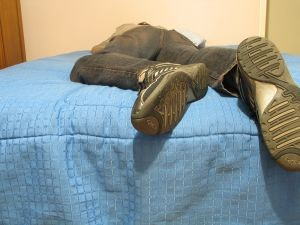
\includegraphics[width=0.3\textwidth]{./figure/shoes.jpg}
\hspace{1cm}
$\Longrightarrow$
\hspace{1cm}
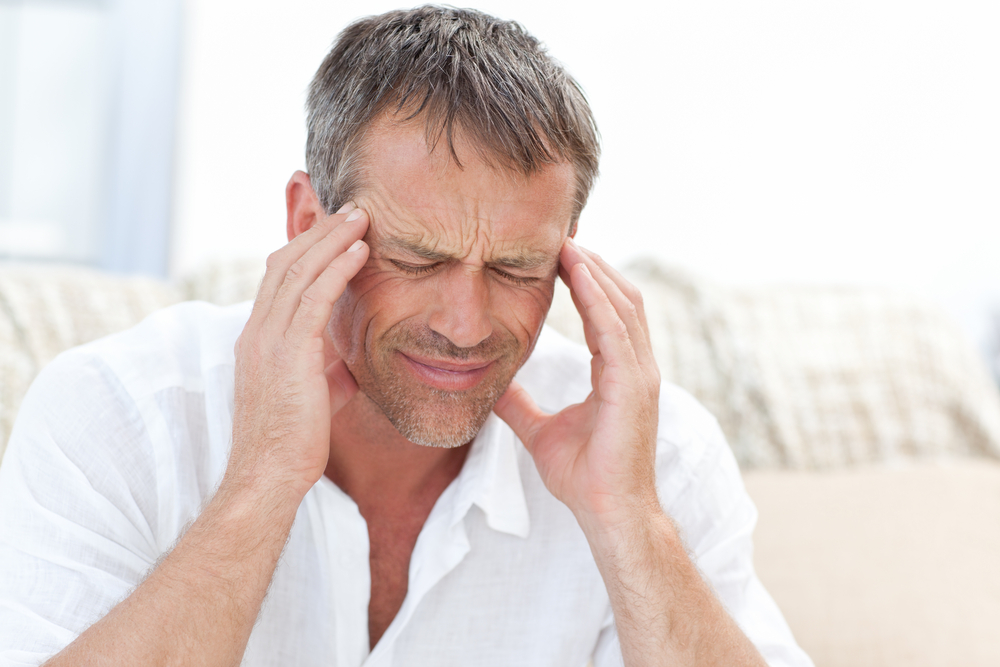
\includegraphics[width=0.3\textwidth]{./figure/headache.jpg}
\end{center}

\pause He then posits the following \blue{causal} relationship:
\begin{itemize}
  \pause \item \blue{Explanatory variable}: sleeping with shoes on 
 \item \blue{Response variable}: waking up with headaches
\end{itemize}

\pause What's wrong with hypotheses?
\end{frame}
%------------------------------------------------------------------------------




\end{document}




